\documentclass[conference]{IEEEtran}
\usepackage{amsmath,graphicx,url}
\begin{document}
\title{Reproducible Transformer Based Handwritten Text Recognition with Page Segmentation and Model Diagnostics}
\author{\IEEEauthorblockN{Dr. A Malikarjun reddy}\IEEEauthorblockA{HOD, Artificial intelligence\\ and machine learning}\and\IEEEauthorblockN{B. Purushowtham sai}\IEEEauthorblockA{Artificial intelligence\\ and machine learning}\and\IEEEauthorblockN{T. Manavi rao}\IEEEauthorblockA{Artificial intelligence\\ and machine learning}}
\maketitle
\begin{abstract}
Turning a handwritten page into editable text involves two linked tasks: locating its lines and recognizing their content. This study develops an English transcription workflow using a pretrained TrOCR-small recognizer, image preprocessing, page segmentation, and an interface for reviewing the output. Decoder fine-tuning is evaluated using 6482 IAM training lines, 256 validation lines, and 512 test lines on a Tesla T4. The corrected experiment preserves the checkpoint's original decoder start token. On the selected test set, the pretrained model achieves a character error rate of 5.92\% and a word error rate of 13.63\%. The adapted checkpoint, selected by validation character error rate, yields 22.81\% and 38.16\%, respectively. Although training loss falls, transcription quality declines. The study documents this negative result and the decisions needed to separate a working application from a valid evaluation. It introduces no new recognition architecture. Complete-page accuracy and generalization to independently collected handwriting remain to be established.
\end{abstract}
\begin{IEEEkeywords}handwritten text recognition, TrOCR, IAM, transfer learning\end{IEEEkeywords}
\section{Introduction}
A handwritten page contains more than a sequence of characters. Before recognition can begin, a system must identify the text lines and preserve their reading order. Uneven spacing, skew, faint strokes, and page rules can disrupt this process. A usable transcription tool should therefore let readers inspect the detected lines and correct the resulting text.

Pretrained recognizers provide a useful starting point for this task [1]. Adapting one to a particular dataset still requires evidence that the adaptation helps. Changes to image preparation, target sequences, and decoding can affect the final transcript even when the training objective decreases. Evaluation must measure the text that the model actually generates.

The present work connects dataset export, image preparation, line recognition, page segmentation, and manual review in one workflow. It also compares the original model with a decoder adapted on IAM lines. The comparison reveals a loss of recognition quality after fine-tuning. Reporting that result is central to the study: the implementation demonstrates a practical workflow, but the experiment does not support an accuracy-improvement claim.
\section{Background and Data}
TrOCR uses a transformer image encoder and an autoregressive text decoder [1]. We use microsoft/trocr-small-handwritten, a public checkpoint previously fine-tuned on IAM for recognition of individual text lines [2]. Its configuration specifies a 12-layer DeiT encoder, a hidden size of 384, 384 by 384 input images, and 16 by 16 patches. The decoder has six layers and a vocabulary of 64044 entries.


Each selected record includes its transcription, source split, row index, image paths, and SHA-256 pixel hash. The export saves decoded RGB images and their processed versions. Here, raw refers to the decoded images before our preprocessing; it does not mean the original IAM archive bytes. The export also checks exact image duplicates and records exclusions. It identifies the data selected for this experiment without claiming to reproduce the checkpoint's entire pretraining history.

The mirror lacks writer identifiers, so writer separation cannot be independently checked in this implementation. Prior IAM exposure in the starting checkpoint also limits conclusions about generalization. The scores should be read as results on this IAM sample. Users of the original database must observe its non-commercial research terms and registration and citation requirements [5].
\section{Preprocessing and Page Recognition}
Image preparation first applies EXIF orientation and places transparent pixels on a white background. It then converts the image to grayscale, applies autocontrast with a 0.2\% cutoff, and restores RGB format. The saved TrOCR processor handles resizing and normalization. The training set receives no synthetic samples or augmentation.

For page input, a thumbnail operation limits the image to 2400 by 3400 pixels while preserving its aspect ratio. Otsu thresholding creates a foreground mask. Morphological opening detects long horizontal and vertical rules, which are removed from this mask to aid segmentation. The recognizer receives crops from the deskewed image, so this mask operation does not erase strokes in the recognition input.

Deskewing searches angles from -5 to +5 degrees in steps of 0.5 degrees on a reduced mask. The selected angle maximizes the sum of squared horizontal row projections. Components smaller than six pixels are suppressed, and vertical closing with a seven-pixel kernel links nearby active rows into bands. Small margins are added to the resulting boxes before they are sorted from top to bottom.

Each crop is decoded greedily with one beam and a limit of 128 new tokens. The line transcripts are joined with newline characters. Saved outputs include the text, deskewed image, crops, and boxes expressed in the resized, deskewed coordinate system. This heuristic is intended for clean, upright English pages with one text column. Multiple columns, tables, overlapping lines, and strong perspective distortion fall outside the evaluated workflow.
\section{Training and Evaluation}
Training uses a Tesla T4, float32 computation, batches of eight, and three epochs. The encoder remains frozen in evaluation mode while AdamW updates the decoder. The learning rate is 0.00001, weight decay is 0.01, and gradients are clipped at norm 1. Padding in the target labels is replaced with -100 so that it does not contribute to cross-entropy loss. Optimizer state is not retained for exact recovery of an interrupted run.

After each epoch, validation character error rate determines whether to select the checkpoint. The selected model and the original pretrained model are evaluated on the same 512 test lines. Test performance is not used to choose an epoch. A single seed is used, so these measurements do not establish variability across repeated runs.

An initial implementation changed the decoder start token from the checkpoint's identifier 2 to the tokenizer classification identifier 0. That change made the initial baseline unsuitable for comparison. The corrected experiment restarts from the public weights and preserves identifier 2. Only this corrected experiment contributes to the main results. Other aspects of target construction still require a controlled check; correcting one configuration error does not validate every decoder convention.

Evaluation normalizes whitespace while preserving letter case and punctuation. Equations (1) and (2) define corpus character error rate (CER) and word error rate (WER). Exact-line accuracy is the fraction of complete normalized lines that match the reference. Insertions can make an error rate exceed 100\%. Loss is reported as a sample-weighted average of batch token losses and should not be interpreted as transcription accuracy.
\begin{equation}\mathrm{CER}=\frac{S_c+D_c+I_c}{N_c}\end{equation}\begin{equation}\mathrm{WER}=\frac{S_w+D_w+I_w}{N_w}\end{equation}
\section{Results}
Table I reports the corrected test comparison. The original checkpoint reaches 5.9206\% CER, 13.6304\% WER, and 40.8203\% exact-line accuracy. The selected adapted checkpoint reaches 22.8084\% CER, 38.1608\% WER, and 2.7344\% exact-line accuracy. Fine-tuning therefore raises CER by 16.8878 percentage points and WER by 24.5304 percentage points on this sample.

Training loss falls from 2.7403 in epoch one to 1.3524 and 1.0371 in epochs two and three. Validation CER moves in the opposite direction: 19.0260\%, 22.9864\%, and 28.4185\%. Validation WER likewise rises from 32.9987\% to 40.5270\% and 48.4734\%. The selection rule consequently chooses epoch one. As Fig. 1 illustrates, a lower training loss does not correspond to a better generated transcript in this run.

The recorded interval of 692.7 seconds covers baseline evaluation through final test evaluation. Dataset download, image export, archive creation, and interface startup are outside that interval. It is neither an end-to-end runtime measurement nor a page-recognition latency result. A page assembled from four test-line images checks whether the workflow runs, but supplies no evidence of accuracy on naturally written pages.
\begin{table}[ht]\centering\caption{Corrected run test results}\begin{tabular}{lrrr}\hline Model & CER (\%) & WER (\%) & Exact (\%)\\\hline Pretrained & 5.9206 & 13.6304 & 40.8203\\ Fine-tuned & 22.8084 & 38.1608 & 2.7344\\\hline\end{tabular}\end{table}
\begin{figure}[ht]\centering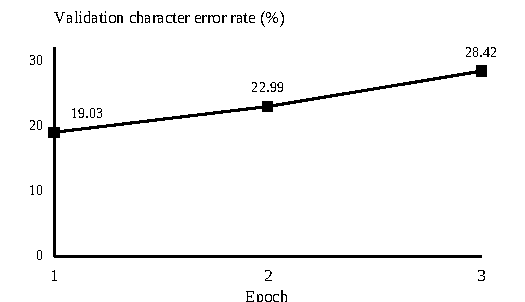
\includegraphics[width=\columnwidth]{validation_curve.pdf}\caption{Validation CER increases after the first epoch.}\end{figure}
\section{Interface and Deployment}
The Ink and Type interface accepts page images and individual line images. Users can inspect detected boxes and crops, edit the recognized text, and download the revision. A results view presents the measured model metrics. These controls make missing or merged lines easier to identify. The interface does not display an uncalibrated score as a probability that the text is correct.

The local application uses the original pretrained checkpoint because it performs better in the measured comparison. Its output must therefore be distinguished from the adapted model's results. Functional checks cover blank input, empty pages, image-size limits, export of edited text, and recognition of an actual test-line image. Such checks establish application behavior, not general recognition accuracy.

Artifact recovery is a further limitation. Saved notebook output preserves the corrected measurements, but the corresponding selected weights were not recovered locally after the Colab runtime expired. A recovered archive contains the earlier misconfigured model and cannot substantiate the corrected model's scores. The application stores the original pretrained weights separately, and the saved metrics identify which experiment they describe.
\section{Discussion and Limitations}
The divergence between training loss and validation error shows why adaptation should be judged by generated text. Restoring the original decoder start token produces a plausible baseline, but the corrected fine-tuning still degrades recognition. Possible causes include further adaptation of an already IAM-trained model, sensitivity to image preparation, target-sequence construction, and the optimization settings. This experiment does not isolate their individual effects.

The next controlled experiment should trace one sample through its target tokens, shifted decoder inputs, and first predicted token. Subsequent ablations should examine the original image processor, a smaller learning rate, and alternative choices of trainable layers. The unchanged checkpoint should also be eligible for validation-based selection. These decisions should use validation data rather than repeated inspection of the present test sample.

The study includes no repeated seeds, confidence intervals, statistical significance test, or systematic human error analysis. Writer independence remains unverified, and prior IAM exposure restricts the interpretation of the baseline. Line-level scores also omit segmentation and reading-order errors. Close spacing, rules, shadows, skew, and the generation limit may cause missing, merged, misplaced, or truncated text. Independently transcribed pages are needed to measure complete-page CER and WER, line recall, and reading order.
\section{Conclusion}
This work implements an inspectable English handwriting transcription workflow and records a negative fine-tuning result. On the selected IAM test lines, the original pretrained model outperforms the adapted checkpoint chosen by validation CER. The interface supports review and correction, while the evaluation identifies what has and has not been measured. Further work should verify decoder targets, test adaptation choices under controlled conditions, and evaluate real pages with independent ground truth. Until that evidence is available, retaining the stronger baseline is the supported deployment choice.
\begin{thebibliography}{5}
\bibitem{r1} M. Li et al., TrOCR: Transformer-based Optical Character Recognition with Pre-trained Models, arXiv:2109.10282, 2021, doi: 10.48550/arXiv.2109.10282.
\bibitem{r2} Microsoft, TrOCR small handwritten model card. [Online]. Available: https://huggingface.co/microsoft/trocr-small-handwritten. Accessed: Oct. 16, 2026.
\bibitem{r3} U.-V. Marti and H. Bunke, The IAM-database: An English sentence database for offline handwriting recognition, International Journal on Document Analysis and Recognition, vol. 5, pp. 39-46, 2002, doi: 10.1007/s100320200071.
\bibitem{r4} Teklia, IAM line dataset. [Online]. Available: https://huggingface.co/datasets/Teklia/IAM-line. Accessed: Oct. 16, 2026.
\bibitem{r5} Computer Vision and Artificial Intelligence Group, IAM Handwriting Database, HEIA-FR. [Online]. Available: https://fki.tic.heia-fr.ch/databases/iam-handwriting-database. Accessed: Oct. 16, 2026.
\end{thebibliography}
\end{document}
